\documentclass[11pt,compress,t,notes=noshow, xcolor=table]{beamer}
\usepackage[]{graphicx}\usepackage[]{color}
% maxwidth is the original width if it is less than linewidth
% otherwise use linewidth (to make sure the graphics do not exceed the margin)
\makeatletter
\def\maxwidth{ %
  \ifdim\Gin@nat@width>\linewidth
    \linewidth
  \else
    \Gin@nat@width
  \fi
}
\makeatother

\newcommand{\citebutton}[2]{%
\beamergotobutton{\href{#2}{#1}}%
}

\newcommand{\blu}[1]{\textcolor{blue}{#1}}
\newcommand{\org}[1]{\textcolor{orange}{#1}}
\newcommand{\ques}{\textbf{\textcolor{red}{Question:  }}}
\newcommand{\questionssofar}{\begin{frame}\frametitle{Any questions?}\end{frame}}

\newcommand\warning{%
 \makebox[1.4em][c]{%
 \makebox[0pt][c]{\raisebox{.1em}{\scriptsize!}}%
 \makebox[0pt][c]{\color{red}\normalsize$\bigtriangleup$}}}%

\definecolor{fgcolor}{rgb}{0.345, 0.345, 0.345}
\newcommand{\hlnum}[1]{\textcolor[rgb]{0.686,0.059,0.569}{#1}}%
\newcommand{\hlstr}[1]{\textcolor[rgb]{0.192,0.494,0.8}{#1}}%
\newcommand{\hlcom}[1]{\textcolor[rgb]{0.678,0.584,0.686}{\textit{#1}}}%
\newcommand{\hlopt}[1]{\textcolor[rgb]{0,0,0}{#1}}%
\newcommand{\hlstd}[1]{\textcolor[rgb]{0.345,0.345,0.345}{#1}}%
\newcommand{\hlkwa}[1]{\textcolor[rgb]{0.161,0.373,0.58}{\textbf{#1}}}%
\newcommand{\hlkwb}[1]{\textcolor[rgb]{0.69,0.353,0.396}{#1}}%
\newcommand{\hlkwc}[1]{\textcolor[rgb]{0.333,0.667,0.333}{#1}}%
\newcommand{\hlkwd}[1]{\textcolor[rgb]{0.737,0.353,0.396}{\textbf{#1}}}%
\let\hlipl\hlkwb

\usepackage{framed}
\makeatletter
\newenvironment{kframe}{%
 \def\at@end@of@kframe{}%
 \ifinner\ifhmode%
  \def\at@end@of@kframe{\end{minipage}}%
  \begin{minipage}{\columnwidth}%
 \fi\fi%
 \def\FrameCommand##1{\hskip\@totalleftmargin \hskip-\fboxsep
 \colorbox{shadecolor}{##1}\hskip-\fboxsep
     % There is no \\@totalrightmargin, so:
     \hskip-\linewidth \hskip-\@totalleftmargin \hskip\columnwidth}%
 \MakeFramed {\advance\hsize-\width
   \@totalleftmargin\z@ \linewidth\hsize
   \@setminipage}}%
 {\par\unskip\endMakeFramed%
 \at@end@of@kframe}
\makeatother

\definecolor{shadecolor}{rgb}{.97, .97, .97}
\definecolor{messagecolor}{rgb}{0, 0, 0}
\definecolor{warningcolor}{rgb}{1, 0, 1}
\definecolor{errorcolor}{rgb}{1, 0, 0}
\newenvironment{knitrout}{}{} % an empty environment to be redefined in TeX

\usepackage{alltt}
\newcommand{\SweaveOpts}[1]{}  % do not interfere with LaTeX
\newcommand{\SweaveInput}[1]{} % because they are not real TeX commands
\newcommand{\Sexpr}[1]{}       % will only be parsed by R
\newcommand{\xmark}{\ding{55}}%


\usepackage[english]{babel}
\usepackage[utf8]{inputenc}

\usepackage{dsfont}
\usepackage{verbatim}
\usepackage{amsmath}
\usepackage{amsfonts}
\usepackage{amssymb}
\usepackage{bm}
\usepackage{csquotes}
\usepackage{multirow}
\usepackage{longtable}
\usepackage{booktabs}
\usepackage{enumerate}
\usepackage[absolute,overlay]{textpos}
\usepackage{psfrag}
\usepackage{algorithm}
\usepackage{algpseudocode}
\usepackage{eqnarray}
\usepackage{arydshln}
\usepackage{tabularx}
\usepackage{placeins}
\usepackage{tikz}
\usepackage{setspace}
\usepackage{colortbl}
\usepackage{mathtools}
\usepackage{wrapfig}
\usepackage{bm}
\usepackage{amsmath}
\usepackage{pifont}

\usetikzlibrary{shapes.multipart,shapes,arrows,automata,positioning,calc,chains,trees, shadows}
\tikzset{
  %Define standard arrow tip
  >=stealth',
  %Define style for boxes
  punkt/.style={
    rectangle,
    rounded corners,
    draw=black, very thick,
    text width=6.5em,
    minimum height=2em,
    text centered},
  % Define arrow style
  pil/.style={
    ->,
    thick,
    shorten <=2pt,
    shorten >=2pt,}
}

\tikzstyle{vec}=[draw, rectangle, fill = white, minimum width=5mm, minimum height=1cm, inner sep = 2pt]

\usepackage{subfig}

% Defines macros and environments
\usepackage{../../style/lmu-lecture}


\let\code=\texttt
\let\proglang=\textsf

\setkeys{Gin}{width=0.9\textwidth}

\setbeamertemplate{frametitle}{\expandafter\uppercase\expandafter\insertframetitle}

\usepackage{bbm}
% basic latex stuff
\newcommand{\pkg}[1]{{\fontseries{b}\selectfont #1}} %fontstyle for R packages
\newcommand{\lz}{\vspace{0.5cm}} %vertical space
\newcommand{\dlz}{\vspace{1cm}} %double vertical space
\newcommand{\oneliner}[1] % Oneliner for important statements
{\begin{block}{}\begin{center}\begin{Large}#1\end{Large}\end{center}\end{block}}


%new environments
\newenvironment{vbframe}  %frame with breaks and verbatim
{
 \begin{frame}[containsverbatim,allowframebreaks]
}
{
\end{frame}
}

\newenvironment{vframe}  %frame with verbatim without breaks (to avoid numbering one slided frames)
{
 \begin{frame}[containsverbatim]
}
{
\end{frame}
}

\newenvironment{blocki}[1]   % itemize block
{
 \begin{block}{#1}\begin{itemize}
}
{
\end{itemize}\end{block}
}

\newenvironment{fragileframe}[2]{  %fragile frame with framebreaks
\begin{frame}[allowframebreaks, fragile, environment = fragileframe]
\frametitle{#1}
#2}
{\end{frame}}


\newcommand{\myframe}[2]{  %short for frame with framebreaks
\begin{frame}[allowframebreaks]
\frametitle{#1}
#2
\end{frame}}

\newcommand{\remark}[1]{
  \textbf{Remark:} #1
}


\newenvironment{deleteframe}
{
\begingroup
\usebackgroundtemplate{
\includegraphics[width=\paperwidth,height=\paperheight]{../style/color/red.png}}
 \begin{frame}
}
{
\end{frame}
\endgroup
}
\newenvironment{simplifyframe}
{
\begingroup
\usebackgroundtemplate{
\includegraphics[width=\paperwidth,height=\paperheight]{../style/color/yellow.png}}
 \begin{frame}
}
{
\end{frame}
\endgroup
}\newenvironment{draftframe}
{
\begingroup
\usebackgroundtemplate{
\includegraphics[width=\paperwidth,height=\paperheight]{../style/color/green.jpg}}
 \begin{frame}
}
{
\end{frame}
\endgroup
}
% https://tex.stackexchange.com/a/261480: textcolor that works in mathmode
\makeatletter
\renewcommand*{\@textcolor}[3]{%
  \protect\leavevmode
  \begingroup
    \color#1{#2}#3%
  \endgroup
}
\makeatother





\input{../../latex-math/basic-math.tex}
\input{../../latex-math/basic-ml.tex}

\newcommand{\titlefigure}{figure/transformer_sq.png}
\newcommand{\learninggoals}{
\item Understand Masked Self-Attention and the role of causality in decoding
\item Understand the connection between the encoder and the decoder}

\title{Transformer}
% \author{Bernd Bischl, Christoph Molnar, Daniel Schalk, Fabian Scheipl}
\institute{\href{https://slds-lmu.github.io/lecture_dl4nlp/}{slds-lmu.github.io/lecture\_dl4nlp}}
\date{}

\begin{document}
\lecturechapter{The Decoder}
\lecture{Deep Learning for NLP}

% ------------------------------------------------------------------------------

\begin{vbframe}{RNNs for autoregressive LM \& decoding}

\vfill

\begin{itemize}
\item In autoregressive language modeling, or in the decoder of a sequence-to-sequence model, the task is to always predict the next word
\item In an RNN, a given state $\vec h^{(j)}$ depends on past inputs $x^{(1)} \ldots x^{(j)}$
\item Thus, the RNN is unable to ``cheat'':
\end{itemize}
\begin{center}
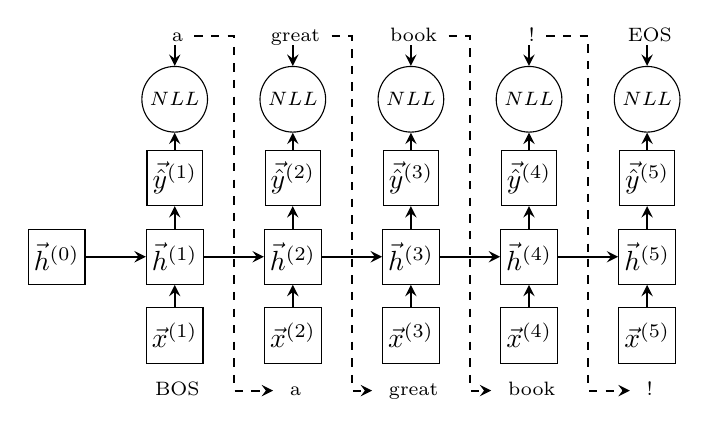
\begin{tikzpicture}
\node (h0) [vec, minimum height=7mm] at (0, 1) {$\vec h^{(0)}$};
\foreach \i/\word in {1/BOS,2/a,3/great,4/book,5/!}{
\node (h\i) [vec, minimum height=7mm] at (\i*1.5, 1) {$\vec h^{(\i)}$};
\node (yhat\i) [vec, minimum height=7mm] at (\i*1.5, 2) {$\vec {\hat{y}}^{(\i)}$};
\node (nll\i) [draw, circle, inner sep=2pt] at (\i*1.5, 3) {\scriptsize $NLL$};
\node (e\i) [vec, minimum height=7mm] at (\i*1.5, 0) {$\vec x^{(\i)}$};
}
\foreach \i/\word in {1/BOS,2/a,3/great,4/book,5/!}{
\node (w\i) [font=\scriptsize, inner sep=0] at (\i*1.5, -.7) {\phantom{A}\word\phantom{g}};
}

\foreach \i/\word in {1/a,2/great,3/book,4/!, 5/EOS}{
\node (y\i) [font=\scriptsize, inner sep=0] at (\i*1.5, 3.8) {\phantom{A}\word\phantom{g}};
}

\foreach \i/\j in {0/1, 1/2, 2/3, 3/4, 4/5}{
\draw [->, >=stealth, thick] (h\i) -- (h\j);
\draw [->, >=stealth, thick] (e\j) -- (h\j);
\draw [->, >=stealth, thick] (h\j) -- (yhat\j);
\draw [->, >=stealth, thick] (yhat\j) -- (nll\j);
\draw [->, >=stealth, thick] (y\j) -- (nll\j);
} 
\foreach \i/\j in {1/2, 2/3, 3/4, 4/5}{
\node at ($(h\i)!0.5!(h\j)$) [inner sep=0pt] (p) {};
\draw [->, >=stealth, thick, dashed] (y\i.east)  --(p|-y\i.east) -- (p) -- (p |- w\j.west) -- (w\j.west);
}
\end{tikzpicture}
\end{center}
\vfill

\end{vbframe}

% ------------------------------------------------------------------------------

\begin{vbframe}{Self-attention for AR LM \& decoding}

\begin{itemize}
\item With attention, all $\vec o_j$ depend on all $\vec v_{j'}$ (and by extension, all $\vec x_{j'}$).
\item This means that the model can easily cheat by looking at future words (red connections)
\end{itemize}
\begin{center}
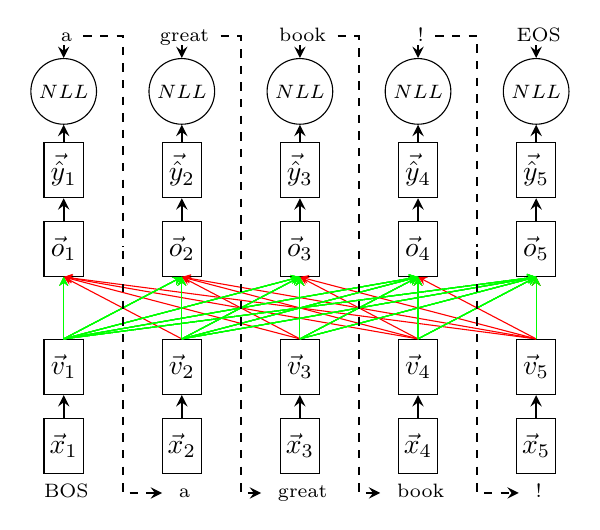
\begin{tikzpicture}
\foreach \i/\word in {1/BOS,2/a,3/great,4/book,5/!}{
\node (h\i) [vec, minimum height=7mm] at (\i*1.5, 1) {$\vec o_\i$};
\node (yhat\i) [vec, minimum height=7mm] at (\i*1.5, 2) {$\vec {\hat{y}}_\i$};
\node (nll\i) [draw, circle, inner sep=2pt] at (\i*1.5, 3) {\scriptsize $NLL$};
\node (e\i) [vec, minimum height=7mm] at (\i*1.5, -.5) {$\vec v_\i$};
\node (x\i) [vec, minimum height=7mm] at (\i*1.5, -1.5) {$\vec x_\i$};
}
\foreach \i/\word in {1/BOS,2/a,3/great,4/book,5/!}{
\node (w\i) [font=\scriptsize, inner sep=0] at (\i*1.5, -2.1) {\phantom{A}\word\phantom{g}};
}

\foreach \i/\word in {1/a,2/great,3/book,4/!, 5/EOS}{
\node (y\i) [font=\scriptsize, inner sep=0] at (\i*1.5, 3.7) {\phantom{A}\word\phantom{g}};
}

\foreach \i/\j in {0/1, 1/2, 2/3, 3/4, 4/5}{
\draw [->, >=stealth, thick] (h\j) -- (yhat\j);
\draw [->, >=stealth, thick] (yhat\j) -- (nll\j);
\draw [->, >=stealth, thick] (y\j) -- (nll\j);
\draw [->, >=stealth, thick] (x\j) -- (e\j);
} 
\foreach \i in {1,2,3,4,5}{
\foreach \j in {\i,...,5}{
\draw [<-, >=stealth, red] (h\i.south) -- (e\j.north);
}
\foreach \i in {1,2,3,4,5}{
\foreach \j in {\i,...,5}{
\draw [->, >=stealth, green] (e\i.north) -- (h\j.south);
}
}
}

\foreach \i/\j in {1/2, 2/3, 3/4, 4/5}{
\node at ($(h\i)!0.5!(h\j)$) [inner sep=0pt] (p) {};
\draw [->, >=stealth, thick, dashed] (y\i.east)  --(p|-y\i.east) -- (p) -- (p |- w\j.west) -- (w\j.west);
}
\end{tikzpicture}
\end{center}

\end{vbframe}

% ------------------------------------------------------------------------------

\begin{vbframe}{Masked self-attention}

\vfill

\begin{itemize}
\item So when we use self-attention for language modeling or in a sequence-to-sequence decoder, we have to prevent $\vec o_j$ from attending to any $\vec v_{j'}$ where $j' > j$.
\item \ques How can we do that?
\item Remember:
$$ \begin{aligned}
\vec o_j & = \sum_{j' = 1}^{J} \alpha_{j,j'} \vec v_{j'} \\
 \alpha_{j,j'} & = \frac{\mathrm{exp}(e_{j,j'})}{\sum_{j'' = 1}^J \mathrm{exp}(e_{j,j''})}
\end{aligned}
$$
\begin{itemize}
\item By hardcoding $e_{j,j'} = -\infty$ when $j' > j$ (in practice, ``$\infty$'' is just a large constant)
\item That way, $\mathrm{exp}(e_{j,j'}) = \alpha_{j,j'} = 0$, so $\vec v_{j'}$ has no impact on $\vec o_j$
\end{itemize}
\end{itemize}

\vfill

\end{vbframe}

% ------------------------------------------------------------------------------

\begin{vbframe}{Parallelized masked self-attention}

\vfill

\begin{itemize}
\item Step 1: Calculate $\vec E$ like we usually would
\item Step 1B:
$$
\begin{aligned}
\vec E^\mathrm{masked} & = \vec E \odot \vec M + \infty\vec M-\infty; \qquad m_{j,j'} = \begin{cases} 1 & \text{ if } j' \leq j \\ 0 & \text{ otherwise} \end{cases}
\end{aligned}
$$
\item Example:
\end{itemize}
$$
\begin{aligned}
\vec E & = \begin{bmatrix} e_{1,1} & e_{1,2} & e_{1,3} \\ e_{2,1} & e_{2,2} & e_{2,3} \\ e_{3,1} & e_{3,2} & e_{3,3} \end{bmatrix}; \qquad \vec M = \begin{bmatrix} 1 & 0 & 0 \\ 1 & 1 & 0 \\ 1 & 1 & 1 \end{bmatrix} \\
\vec E^\mathrm{masked} & = \begin{bmatrix} e_{1,1} & -\infty & -\infty \\ e_{2,1} & e_{2,2} & -\infty \\ e_{3,1} & e_{3,2} & e_{3,3} \end{bmatrix} ; \qquad \vec A^\mathrm{masked} = \begin{bmatrix} 1 & 0 & 0 \\ \alpha_{2,1} & \alpha_{2,2} & 0 \\ \alpha_{3,1} & \alpha_{3,2} & \alpha_{3,3} \end{bmatrix} \\
\vec o_1 = \vec v_1; \qquad & \vec o_2 = \alpha_{2,1} \vec v_1 + \alpha_{2,2} \vec v_2; \qquad \vec o_3 = \alpha_{3,1} \vec v_1 + \alpha_{3,2} \vec v_2 + \alpha_{3,3} \vec v_3
\end{aligned}
$$

\vfill

\end{vbframe}

% ------------------------------------------------------------------------------

\begin{vbframe}{AR Transformer at inference time}

\vfill

\begin{itemize}
\item During training (targets known): Use parallelized masked attention 
\item At inference time (targets unknown): Decode prediction in a loop
\item Slower, but at least we don't have to worry about masking anymore
\end{itemize}
\begin{center}
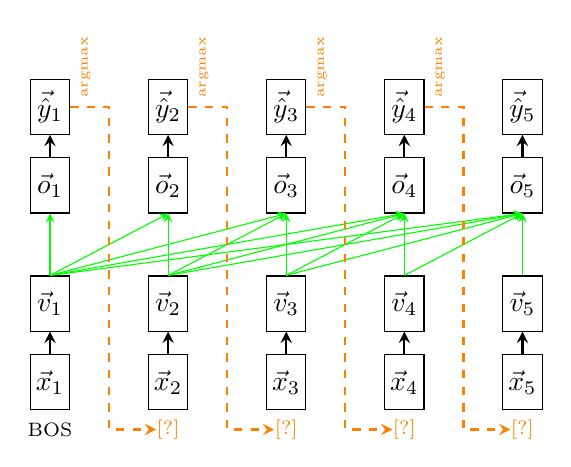
\begin{tikzpicture}
\foreach \i/\word in {1/BOS,2/a,3/great,4/book,5/!}{
\node (h\i) [vec, minimum height=7mm] at (\i*1.5, 1) {$\vec o_\i$};
\node (yhat\i) [vec, minimum height=7mm] at (\i*1.5, 2) {$\vec {\hat{y}}_\i$};
\node (e\i) [vec, minimum height=7mm] at (\i*1.5, -.5) {$\vec v_\i$};
\node (x\i) [vec, minimum height=7mm] at (\i*1.5, -1.5) {$\vec x_\i$};
}
\foreach \i/\word in {2/a,3/great,4/book,5/!}{
\node (w\i) [font=\scriptsize, inner sep=0, orange] at (\i*1.5, -2.1) {[?]};
}
\foreach \i/\word in {1/BOS}{
\node (w\i) [font=\scriptsize, inner sep=0] at (\i*1.5, -2.1) {BOS};
}

\foreach \i/\j in {0/1, 1/2, 2/3, 3/4, 4/5}{
\draw [->, >=stealth, thick] (h\j) -- (yhat\j);
\draw [->, >=stealth, thick] (x\j) -- (e\j);
} 
\foreach \i in {1,2,3,4,5}{
\foreach \j in {\i,...,5}{
\draw [->, >=stealth, green] (e\i.north) -- (h\j.south);
}
}

\foreach \i/\j in {1/2, 2/3, 3/4, 4/5}{
\node at ($(h\i)!0.5!(h\j)$) [inner sep=0pt] (p) {};
\draw [->, >=stealth, thick, dashed, orange] (yhat\i.east)  --(p|-yhat\i.east) -- (p) -- (p |- w\j.west) -- (w\j.west);
\node at ([xshift=2mm, yshift=5mm] yhat\i.east) [rotate=90, font=\tiny, orange] {argmax};
}
\end{tikzpicture}
\end{center}

\vfill

\end{vbframe}

% ------------------------------------------------------------------------------

\begin{vbframe}{Add. Subtleties: Residual connections}

\vfill

\begin{itemize}
\item Let $\mathcal{F}$ be a function with parameters $\theta$
\item $\mathcal{F}$ with a residual connection:
$$\mathcal{F}'(\vec X; \theta) = \mathcal{F}(\vec X; \theta) + \vec X$$
\begin{center}
\vfill
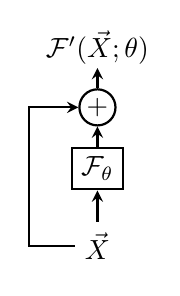
\begin{tikzpicture}[->, >=stealth, thick]
\node (layer) at (0,0) [draw, rectangle, minimum size = 5mm] {$\mathcal{F}_\theta$};
\node (h) [above=1cm of layer, inner sep=1pt] {$\mathcal{F}'(\vec X; \theta)$};
\node (plus) [draw, circle, inner sep=1pt] at ($(layer.north)!0.5!(h.south)$) {$+$};
\node (left) [left=5mm of layer, inner sep=0pt] {};
\node (x) [below=4mm of layer] {$\vec X$};
\draw (x) -- (left |- x) -- (left |- plus) -- (plus);
\draw (x) -- (layer);
\draw (layer) -- (plus);
\draw (plus) -- (h);
\end{tikzpicture}
\end{center}
\item Benefits: Information retention (we add to $\vec X$ but don't replace it) 
\end{itemize}

\vfill

\end{vbframe}

% ------------------------------------------------------------------------------

\begin{vbframe}{Add. Subtleties: Layer normalization}

\vfill

\begin{itemize}
\item Let $\theta = \{\vec \gamma \in \mathbb{R}^d, \vec \beta \in \mathbb{R}^d\}$ be trainable parameters
\item Let $\vec h \in \mathbb{R}^d$ be an output vector of some layer (e.g., an $\vec o_j$ vector from an attention layer)
\item Then layer normalization calculates:
$$ \vec \gamma \odot \frac{\vec h - \mu}{\sigma} + \vec \beta $$
\item where $\mu, \sigma$ are mean and standard deviation over the dimensions of $\vec h$:
$$ \mu = \frac{1}{d} \sum_{i=1}^d h_{i}; \qquad \sigma = \sqrt{\frac{1}{d} \sum_{i=1}^d (h_i - \mu)^2} $$
\item Benefits: Allows us to normalize vectors after every layer; helps against exploding activations on the forward pass
\item In the Transformer, layer normalization is applied position-wise, i.e., every $\vec o_j$ is normalized independently
\end{itemize}

\vfill

\end{vbframe}

% ------------------------------------------------------------------------------

\begin{vbframe}{Encoder-Decoder Attention}

\vfill

\textbf{Open question: How do we connect encoder and decoder?}\\

\vspace{.3cm}
	
Construction of one decoder block:

\vspace{.3cm}
	
	\begin{enumerate}
		\item Masked (Multi-Head) Attention layer (only target sequence)
		\item "Ordinary" (Multi-Head) Attention layer
			\begin{itemize}
				\item Queries from the previous decoder layer
				\item Keys, Values from the encoder output
			\end{itemize}
		\item Feed-Forward layer (w/ residual connections \& layer norm)
	\end{enumerate}
	
\vspace{.3cm}
	
$\to$ Allows the decoder to attend to \textit{all} tokens from the input sequences\\
(cf. Bahdanau et al. (2014) for RNNs)

\vfill

\end{vbframe}

% ------------------------------------------------------------------------------

\begin{vbframe}{The Transformer architecture}

\begin{center}
\begin{tikzpicture}[->, >=stealth, thick, font=\scriptsize]
\node (transformer) at (0,0) {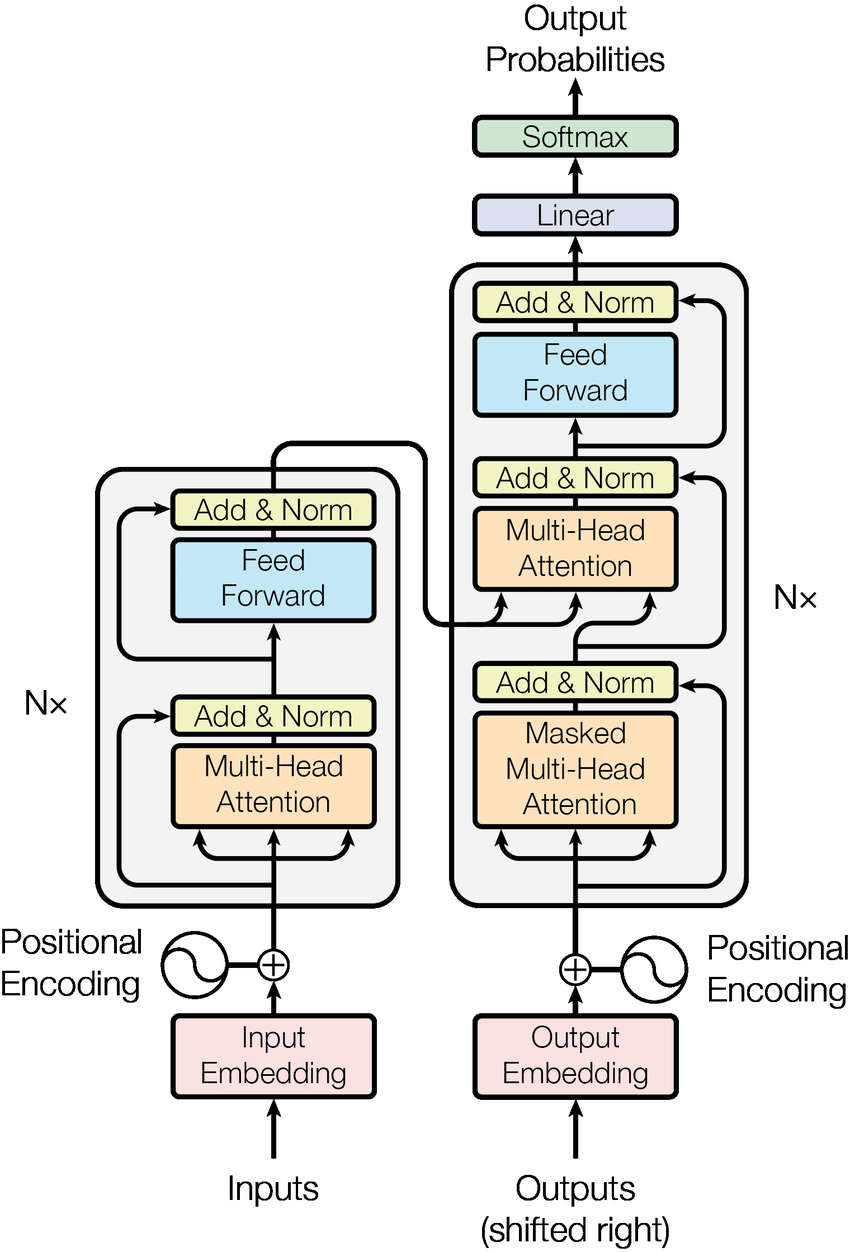
\includegraphics[width=.4\textwidth]{figure/transformer.png}};
\node (enc) [left=2mm of transformer, rotate=90] {encoder};
\node (dec) [right=2mm of transformer, rotate=270] {decoder};
\node (x) [above left=1cm of transformer.south west] {$X$ (source)};
\node (y) [above right=1cm of transformer.south east] {$Y$ (target)};
\draw (x) -- ([yshift=5mm, xshift=1cm] transformer.south west);
\draw (y) -- ([yshift=5mm, xshift=-1cm] transformer.south east);
\node (nll) [draw, circle] at ([yshift=-5mm] transformer.north east) {NLL};
\draw [bend right=55] (y.north east) to (nll);
\draw ([xshift=-1cm, yshift=-5mm] transformer.north east) to (nll);
\node at (-3, 2) [align=left] {(For simpler problems (e.g., \\ classification, tagging), \\ you would simply use \\ the encoder.)};
\end{tikzpicture}
\end{center}
{\tiny Figure from Vaswani et al. 2017: Attention is all you need}

\end{vbframe}

% ------------------------------------------------------------------------------

\endlecture
\end{document}
